%%%%%%%%%%%%%%%%%%%%%%%%%%%%%%%%%%%%%%%%%%%%%%%%%%%%%%%%%%%%%%%%%%%%%
% LaTeX Template: Project Titlepage Modified (v 0.1) by rcx
%
% Original Source: http://www.howtotex.com
% Date: February 2014
% 
% This is a title page template which be used for articles & reports.
% 
% This is the modified version of the original Latex template from
% aforementioned website.
% 
%%%%%%%%%%%%%%%%%%%%%%%%%%%%%%%%%%%%%%%%%%%%%%%%%%%%%%%%%%%%%%%%%%%%%%

\documentclass[12pt]{report}
%\usepackage[a4paper]{geometry}
%\usepackage[myheadings]{fullpage}
%\usepackage{fancyhdr}
%\usepackage[a4paper,width=150mm,top=25mm,bottom=25mm]{geometry}
\usepackage{fancyhdr}
\pagestyle{fancy}
\fancyhf{}
\usepackage{lastpage}
\usepackage{graphicx, wrapfig, subcaption, setspace, booktabs}
\usepackage[T1]{fontenc}
\usepackage[font=small, labelfont=bf]{caption}
\usepackage{fourier}
\usepackage[protrusion=true, expansion=true]{microtype}
\usepackage[english]{babel}
\usepackage{sectsty}
\usepackage{url, lipsum}
\graphicspath{{./images}}


\newcommand{\HRule}[1]{\rule{\linewidth}{#1}}
\onehalfspacing
\setcounter{tocdepth}{5}
\setcounter{secnumdepth}{5}

%-------------------------------------------------------------------------------
% HEADER & FOOTER
%-------------------------------------------------------------------------------
\pagestyle{fancy}
\fancyhf{}
\setlength\headheight{15pt}
\fancyhead[L]{CP-SCM Experiments}

%-------------------------------------------------------------------------------
% TITLE PAGE
%-------------------------------------------------------------------------------

\begin{document}

\title{ \normalsize \textsc{CPSCM Experiments Report}
		\\ [2.0cm]
		\HRule{0.5pt} \\
		\LARGE \textbf{\uppercase{Cyclic Prefix Single Carrier Modulation Techniques and Experimentation}}
		\HRule{2pt} \\ [0.5cm]
		\normalsize  \vspace*{5\baselineskip}}

\date{}

\author{
		Nicholas Elliott \\
                Guided By - Prof. Behrouz Farhang, Brent Kenney  \\                
Department of Electrical and Computer Engineering\\
University of Utah\\ }

\maketitle

\newpage
\section*{ABSTRACT}

Cyclic Prefix Single Carrier Modulation has theoretical advantages and trade-offs compared with
commonly used OFDM transmission schemes.  MIMO phased array equipment installed at the University of
Utah through the RenewLab POWDER research group allow for implementation and analysis of Cyclic Prefix
fSingle Carrier Modulation techniques.  This report characterizes the requirements and parameters for
OFDM transmission and comprable CPSCM requirements and parameters.  Considerations such as channel equalization, PAPR, channel state information and payload size are addressed or explored.  Additional considerations such as equipment limitations, simplifications compared to actual IEEE specifications, additional scope and general information for future students are also addressed.

\section*{INTRODUCTION}
OFDM is ubiqitous for its efficiency and simplicity in implementation, however, simple modifications using
a single carrier which takes advantage of the simplicity of cyclic prefix channel equalization and reduced PAPR
may outperform OFDM for specific use cases.

Hardware setup and limitations.

Uplink Edge use case. PAPR.

Challenge of phase drift and channel equalization without consistent pilots.\\\\\\

\section*{Conceptual Overview}
\subsection*{Typical OFDM}
\subsection*{Sampling Rate and Bandwidth}
\subsection*{Payload Length and Phase Correction}
\paragraph*{Cyclic Prefix Channel Estimation}
\subsection*{State Space Random Walk Channel Characterization}
\paragraph*{Random Walk Channel Model} 
\section*{Methodology}

\subsection*{Baseline OFDM vs. CPSCM Simulations}
\paragraph*{Sampling Rate not Feasible on Hardware}

\subsection*{Baseline OFDM vs. CPSCM on POWDER}

\section*{Multiple Input Multiple Output(MIMO) technique}
Multiple Input Multiple Output (MIMO) is a cutting edge antenna
technology transmitting multiple data streams on multiple transmitters
to multiple receivers. Multiple antennas are used especially when
the link has Non Line of Sight. MIMO increases the range and data
rates both.
Now the capacity of different antenna systems will be studied in order
to see the dramatic increases in capacity obtained by using MIMO systems. The expressions are approximate, but they give an intuition for
the derived benefits in terms of channel capacity when using multiple
antennas

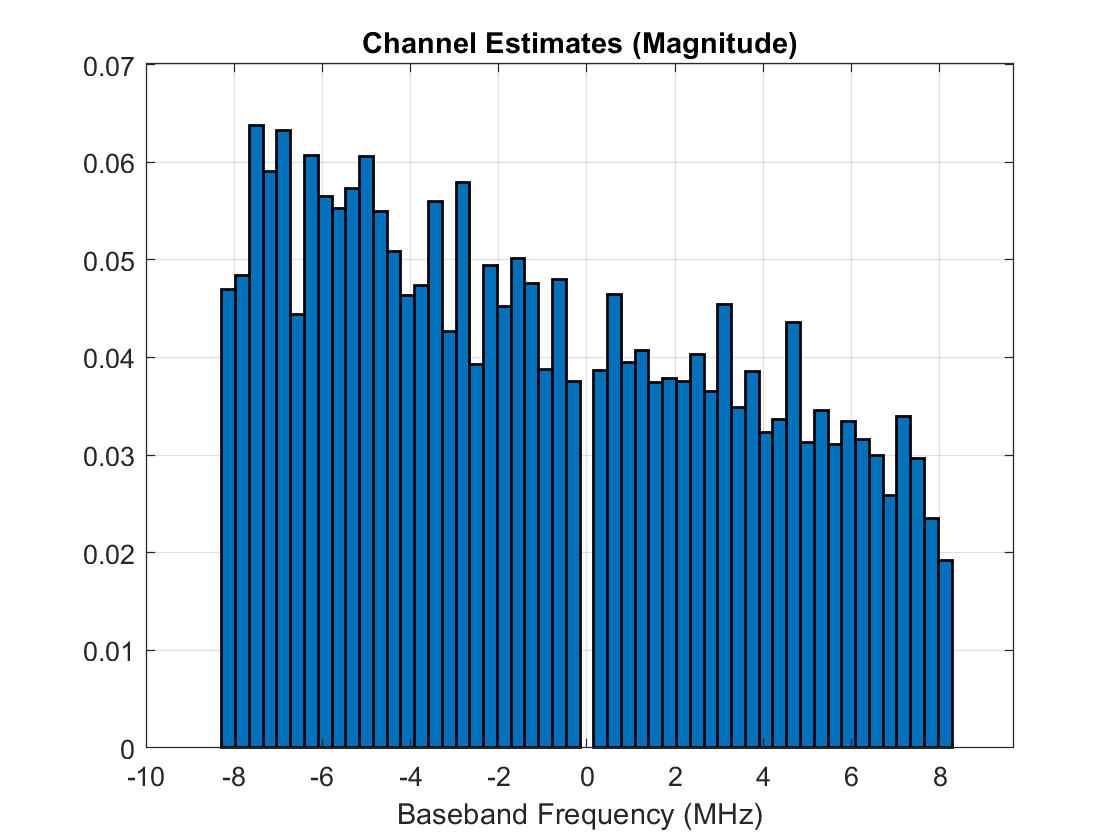
\includegraphics[width=\columnwidth]{channel_est.png}

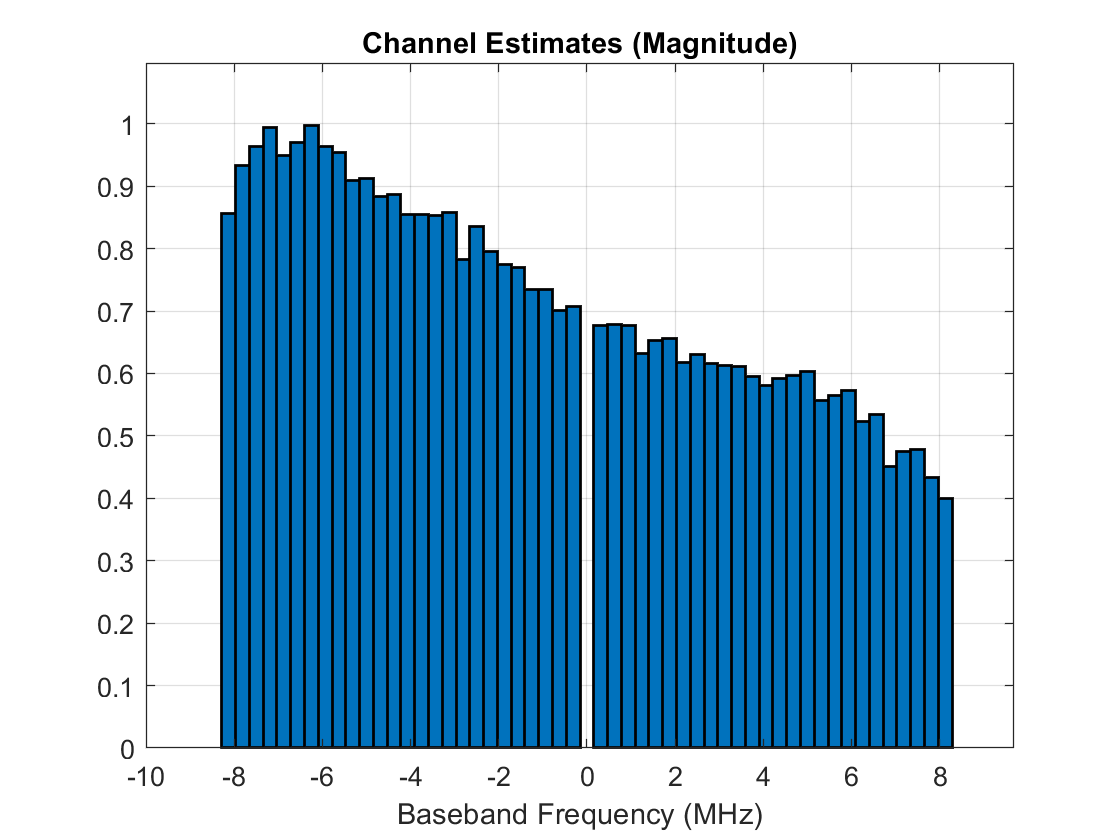
\includegraphics[width=\columnwidth]{CHANNEL_EST_TO_COMPARE_PSD.png}
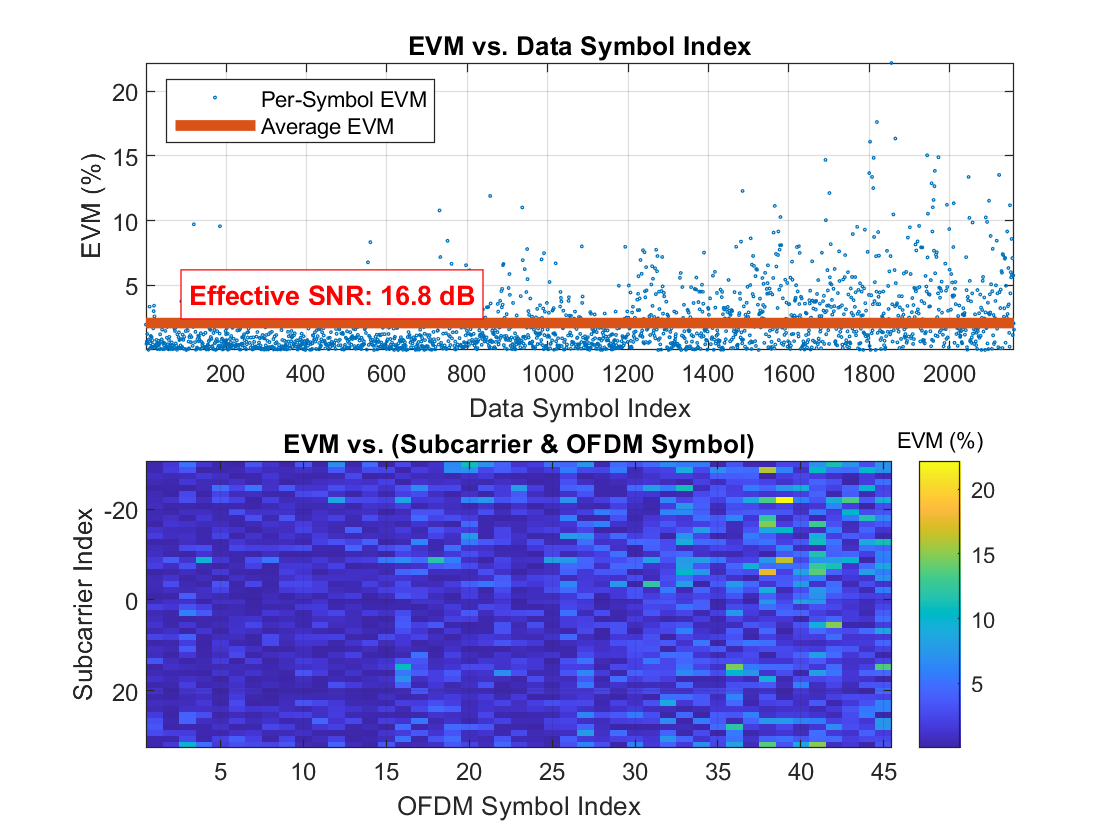
\includegraphics[width=\columnwidth]{EVM_GROWTH_OFDM_16_FRM_45.png}
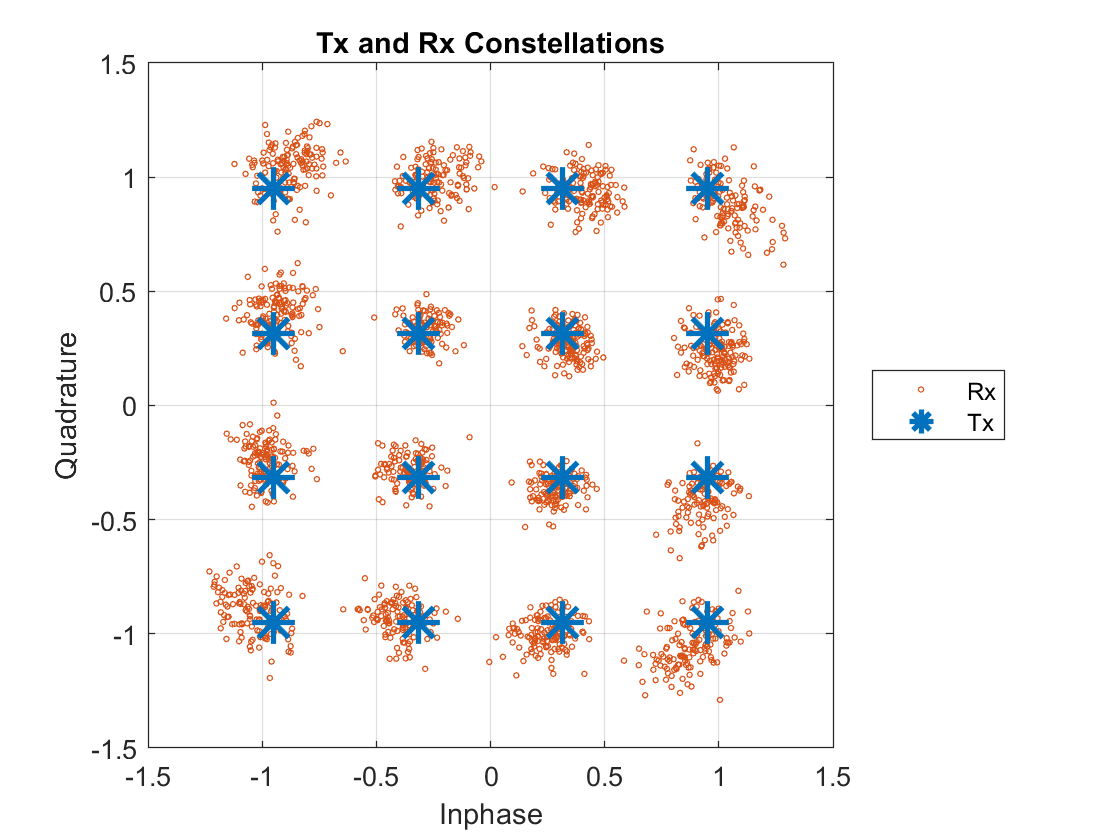
\includegraphics[width=\columnwidth]{phase_drift_OFDM_16QAM_45_FRM.png}
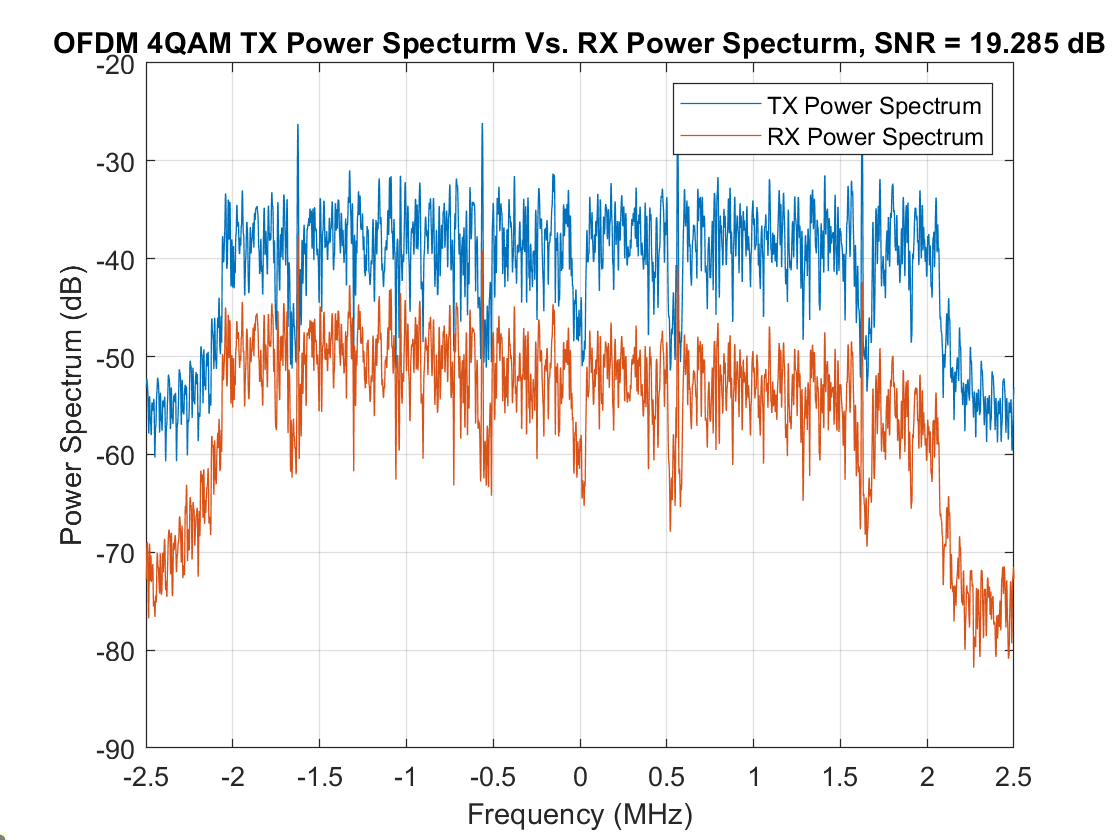
\includegraphics[width=\columnwidth]{RX_VS_TX_PSD.png}

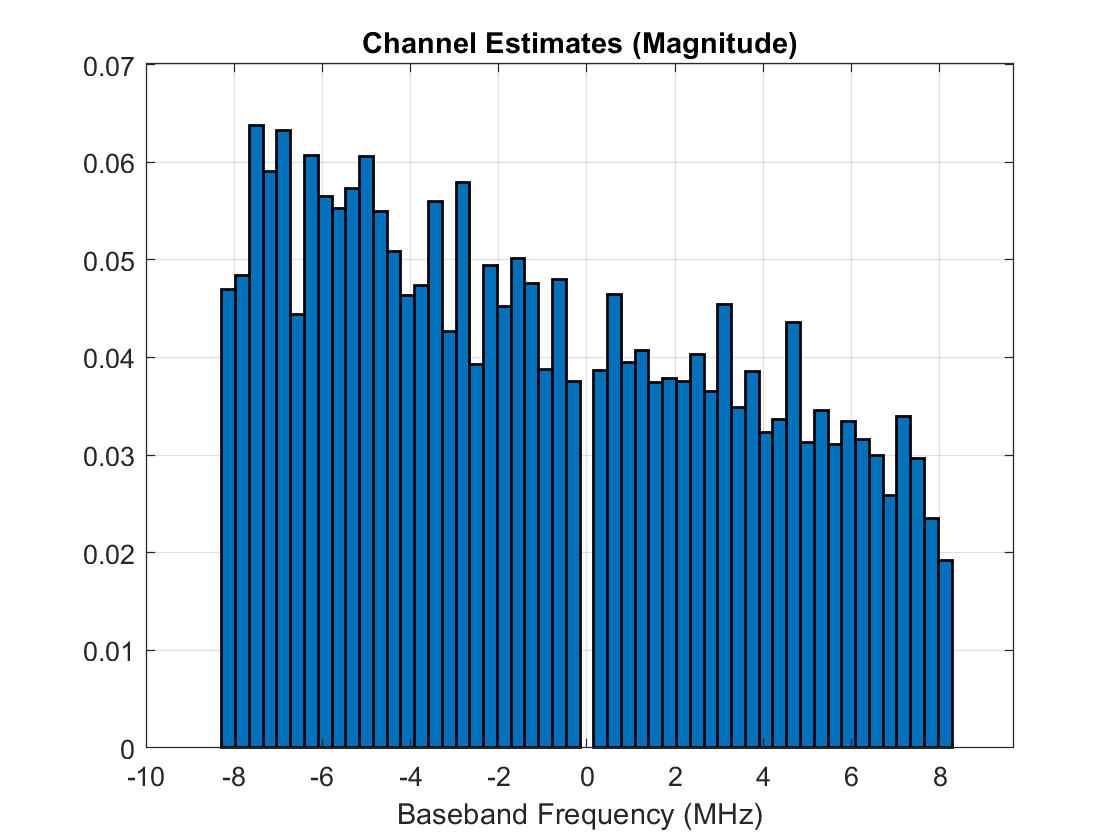
\includegraphics[width=\columnwidth]{channel_est.png}
\section*{Types of smart antenna technology}
\subsection*{Single Input, Single Output}
Assume that for a given channel, whose bandwidth is B, and a given
transmitter power of P the signal at the receiver has an average signal
to noise ratio of SNR.\\
C = B*log2(1 + SNR)

\subsection*{Single Input, Multiple Output}
For the SIMO system, we have NR antennas at the receiver. If the signals
received on these antennas have on average the same amplitude, then
they can be added coherently to produce an NR2 increase in the signal
power. Hence, there is an overall increase in the SNR,\\
Thus, the channel capacity for this channel is approximately equal to\\
C = NR*B*log2(1 + SNR)
\subsection*{Multiple Input, Single Output}
In the MISO system, we have NT transmitting antennas. The total
transmitted power is divided up into the NT transmitter branches. If the
signals add coherently at the receiving antenna we get approximately
an NT fold increase in the SNR as compared to the SISO case. Thus,
the overall increase in SNR is approximately,\\
Channel capacity for this channel is approximately equal to:\\
C = NT*B*log2(1 +SNR)


\begin{figure}[!hbt]
		% Center the figure.
		\begin{center}
		% Include the eps file, scale it such that it's width equals the column width. You can also put width=8cm for example...
%		\includegraphics[width=\columnwidth]{sisosimomiso}
		% Create a subtitle for the figure.
		\caption{SISO, SIMO and MISO system.}
		% Define the label of the figure. It's good to use 'fig:title', so you know that the label belongs to a figure.
		\label{fig:tf_plot}
		\end{center}
	\end{figure}
    \subsection*{Multiple-Input, Multiple-Output}
Different signal transmitted by each antenna, in MIMO using the same
bandwidth and still be able to decode correctly at the receiver. The
capacity of each one of these channels is roughly equal to:\\
C = min(NT,NR)*B*log2(1 +SNR)\\	
Thus, as we can see from , we get a linear increase in capacity with respect to the number of transmitting antennas. So, the key principle at
work here, is that it is more beneficial to transmit data using many different low-powered channels than using one single, high-powered channel.



\section*{MIMO System Model}
Let us consider single user MIMO communication system with 2 antennas at the transmitter and 2 antennas at the receiver. Consider that
we have a transmission sequence is x1; x2;.......... xn. In normal trans-
mission, we send x1 in the first time slot, x2 in the second time slot and
\begin{figure}[!hbt]
		% Center the figure.
		\begin{center}
		% Include the eps file, scale it such that it's width equals the column width. You can also put width=8cm for example...
%		\includegraphics[width=\columnwidth]{mimosys}
		% Create a subtitle for the figure.
		\caption{ MIMO SYSTEM MODEL .}
		% Define the label of the figure. It's good to use 'fig:title', so you know that the label belongs to a figure.
		\label{fig:tf_plot}
		\end{center}
	\end{figure}
xn in the nth time slot. Now we have two transmit antennas, we may
groups the symbols into groups of two. In the first time slot, send x1
and x2 from the first and second antenna. In the second time slot,
send x3 and x4 from the first and second antenna and in next time slot
x5 and x6 and so on. Let us consider for 2x2 MIMO. The signal received
on the first antenna is given by:\\
r1 = h11s1 + h12s2 + n1 \\
The signal received on the second antenna is given by:\\
r2 = h21s1 + h22s2 + n2\\
where, y1 and y2 are the received symbol on the first and second antenna respectively,h11 is the channel from 1st transmit antenna to 1st
receive antenna,h12 is the channel from 2nd transmit antenna to 2nd
receive antenna,h21 is the channel from 1st transmit antenna to 2nd
receive antenna, h22 is the channel from 2nd transmit antenna to 2nd
receive antenna, s1 and s2 are the transmitted symbols and n1 and n2
is the noise on 1st and 2nd receive antennas respectively\\\\\\



    
    \section*{MIMO Advantages}
    The advantages of MIMO based wireless networks are increased range,
throughput and robustness of the data link. This advantage is achieved
by firstly high throughput i.e ability to provide high data rate compared
to range and secondly by using 40MHz channels to increase the available
bandwidth for high data rate.

 \subsection*{1. Better Spectral Efficiency at Low Cost}
 MIMO drives greater bandwidth, reach and spectral efficiency at a lower
cost than the alternative antenna technology.

\subsection*{2. Linear Capacity Growth.}
The MIMO Systems capacity grows linearly with the number of antennas. 2x2 MIMO doubles the capacity and 4x4 MIMO quadruples
capacity.

 \subsection*{3. Backwards compatible.}
Supports both TDD and FDD techniques so can be used with earlier
versions of 802.11x to increase the data rate.

Intel defining the MIMO benefits states MIMO uses multiple transmitter and receiver antennas to allow for increased data throughput
through spatial multiplexing and increased range by exploiting spatial
diversity and this helps in making products that will have Extended
battery life , Expanded wireless connectivity and Immersive entertainment.
\section*{MIMO Disadvantages}
MIMO has very few disadvantages associated with it.\\
The disadvantages of the MIMO system is mostly the need for multiple Antennas the cost of the equipment compared to existing equipment available and limited open source driver support.\\
Computational complexity.\\
Cost for added antennas.\\


    \section*{ ALAMOUTI SPACE-TIME BLOCK CODING}
    Alamouti STBC is a complex space-time diversity
technique that can be used in 2x1 MISO mode or in a 2x2
MIMO mode. It is the only STBC that can achieve its full
diversity gain without needing to sacrifice its data rate.
this property usually gives Alamouti's code a significant
advantage over the higher-order STBCs even though they
achieve a better error-rate performance

\begin{figure}[!hbt]
		% Center the figure.
		\begin{center}
		% Include the eps file, scale it such that it's width equals the column width. You can also put width=8cm for example...
%		\includegraphics[width=\columnwidth]{A}
		% Create a subtitle for the figure.
		\caption{ Alamouti Space Time Diversity .}
		% Define the label of the figure. It's good to use 'fig:title', so you know that the label belongs to a figure.
		\label{fig:tf_plot}
		\end{center}
	\end{figure}
Figure shows that two symbols and their conjugate are
sent, in two time slots, which brings a diversity gain
without having to compromise on the data rate. Over the
air, the transmitted symbols will suffer from channel
fading and noise at the receiver, their sum will be
received. Working principles of 2x1 and 2x2 Alamouti
STBC is indicated Figure respectively.
\subsection*{1) 2x1 Alamouti STBC}
The 2x1 Alamouti STBC systems consists of two antenna
at transmitter and at receiver side contains one antenna as
shown the figure
\begin{figure}[!hbt]
		% Center the figure.
\begin{center}
		% Include the eps file, scale it such that it's width equals the column width. You can also put width=8cm for example...
%		\includegraphics[width=\columnwidth]{B}
		% Create a subtitle for the figure.
		\caption{2X1 Alamouti STBC  .}
		% Define the label of the figure. It's good to use 'fig:title', so you know that the label belongs to a figure.
		\label{fig:tf_plot}
		\end{center}
	\end{figure}
At time t and are transmitted by Transmitter
1 and 2 and after that at time (t+T) their conjugates are
transmitted.
From Table 1 and Figure 4 we can write receiving data;\\
y1 = x1*h1 + x2*h2 + n1  (First time slot) \\
y2 = -x2*h1 + x1*h2 + n2  (Second time slot) \\
Where;
x1 and x2 transmitted data,\\
y1 and y2 received data,\\
h1 and h2 Rayleigh channel,\\
n1 and n2 AWGN noise,\\
In order to get rid of conjugates of transmitted data at the
receiver, we take conjugate of y2;\\
y1 = x1*h1 + x2*h2 + n1\\
y2* = h1*(-x2) + h2*x1 + n2
\subsection*{2) 2x2 Alamouti STBC}
\begin{figure}[!hbt]
		% Center the figure.
\begin{center}
		% Include the eps file, scale it such that it's width equals the column width. You can also put width=8cm for example...
%		\includegraphics[width=\columnwidth]{C}
		% Create a subtitle for the figure.
		\caption{2X2 Alamouti STBC  .}
		% Define the label of the figure. It's good to use 'fig:title', so you know that the label belongs to a figure.
		\label{fig:tf_plot}
		\end{center}
	\end{figure}
    The 2x2 Alamouti STBC System is shown in figure 5
which is similar to 2x1 Alamouti but we have one more
receiver antenna. This system is consists of 2 Transmitter
and 2 Receiver. Working principle is also similar to 2x1
Alamouti. In 2x1 Alamouti we send block codes to just
one receiver but in this system we send block codes to 2
receiver\\
y11 = x1*h11 + x2*h12 + n11 (first timeslot received data in Rx1) \\
y12 = -x2*h11 + x1*h12 + n12 (Second timeslot received data in Rx1)\\
y21 = x1*h21 + x2*h21 + n21 (first timeslot received data in Rx2)\\
 y22 = -x2*h21 + x1*h22 + n22 (Second timeslot received data in Rx2)\\
 Where;
x1 and x2 transmitted data
y11 and y21 are received data (for first time slot)\\
y12 and y22 are received data in (for second time slot)\\
h11,h12 ,h21 ,h22 are Rayleigh channel\\
n11,n12,n21,n22 are AWGN noise\\
Now we take conjugates of y12 , y22 to get rid of
conjugates of transmitted data at the receiver\\
y12* = -x2h11* + x1h12* + n12*\\
y22* = -x2h21* + x1h22* + n22*\\
We write  together to all\\
y11 = x1*h11 + x2*h12 + n11\\
y12* = -x2h11* + x1h12* + n12*\\
y21 = x1*h21 + x2*h21 + n21\\ 
y22* = -x2h21* + x1h22* + n22*\\ \\ \\ \\ \\ 

\section*{Problem Statement:-}
Now days OFDM is used to transmit audio and video over multiple channels . The aim of this project is to analyse behaviour of Image signals/audio signals over a MIMO channel by analysing parameters such as ICI , BER , PSNR , etc.

\section*{Platform :- MATLAB .} 

\section*{Future Plan:-}
In our project  we will transmit the digital image over OFDM and mimo system, find all the parameters like BER , SNR ,etc. using 16-QAM for modulation.


\section*{REFERENCES}
\subsection*{1. "Study and Analysis of 2x2 MIMO Systems for
Different Modulation Techniques using
MATLAB" International Journal of Advanced Research in Computer and Communication Engineering
Vol. 4, Issue 7, July 2015}
\subsection*{2. "Capacity and Performance of MIMO systems for Wireless Communications" Journal of Engineering Science and Technology Review 7 (3) (2014) 108 – 111}
\subsection*{3. "Capacity and Performance Comparison of SISO and MIMO System for Next Generation Network (NGN)" International Journal of Advanced Research in Computer Engineering and Technology (IJARCET)
Volume 3 Issue 9, September 2014}
\subsection*{4. "Dynamic System Performance of SISO, MISO and
MIMO Alamouti Schemes"Dorra Ben Cheikh Battikhy?, Jean-Marc Kelif?, Marceau Coupechouxy and Philippe Godlewskiy
? Orange Labs, Issy-les-moulineaux, France }
\subsection*{5. "OFDM for wireless communication system " Artech House universal personal communications series- Ramaji Prasad}
\subsection*{6."Evaluating the performance of OFDM transceiver for image transfer using
16PSK and 16QAM modulation schemes" International Journal of Scientific Engineering and Technology (ISSN : 2277-1581)
Volume No.3, Issue No.3, pp : 222-226}






    
    
    






\end{document}

%-------------------------------------------------------------------------------
% SNIPPETS
%-------------------------------------------------------------------------------

%\begin{figure}[!ht]
%	\centering
%	\includegraphics[width=0.8\textwidth]{file_name}
%	\caption{}
%	\centering
%	\label{label:file_name}
%\end{figure}

%\begin{figure}[!ht]
%	\centering
%	\includegraphics[width=0.8\textwidth]{graph}
%	\caption{Blood pressure ranges and associated level of hypertension (American Heart Association, 2013).}
%	\centering
%	\label{label:graph}
%\end{figure}

%\begin{wrapfigure}{r}{0.30\textwidth}
%	\vspace{-40pt}
%	\begin{center}
%		\includegraphics[width=0.29\textwidth]{file_name}
%	\end{center}
%	\vspace{-20pt}
%	\caption{}
%	\label{label:file_name}
%\end{wrapfigure}

%\begin{wrapfigure}{r}{0.45\textwidth}
%	\begin{center}
%		\includegraphics[width=0.29\textwidth]{manometer}
%	\end{center}
%	\caption{Aneroid sphygmomanometer with stethoscope (Medicalexpo, 2012).}
%	\label{label:manometer}
%\end{wrapfigure}

%\begin{table}[!ht]\footnotesize
%	\centering
%	\begin{tabular}{cccccc}
%	\toprule
%	\multicolumn{2}{c} {Pearson's correlation test} & \multicolumn{4}{c} {Independent t-test} \\
%	\midrule	
%	\multicolumn{2}{c} {Gender} & \multicolumn{2}{c} {Activity level} & \multicolumn{2}{c} {Gender} \\
%	\midrule
%	Males & Females & 1st level & 6th level & Males & Females \\
%	\midrule
%	\multicolumn{2}{c} {BMI vs. SP} & \multicolumn{2}{c} {Systolic pressure} & \multicolumn{2}{c} {Systolic Pressure} \\
%	\multicolumn{2}{c} {BMI vs. DP} & \multicolumn{2}{c} {Diastolic pressure} & \multicolumn{2}{c} {Diastolic pressure} \\
%	\multicolumn{2}{c} {BMI vs. MAP} & \multicolumn{2}{c} {MAP} & \multicolumn{2}{c} {MAP} \\
%	\multicolumn{2}{c} {W:H ratio vs. SP} & \multicolumn{2}{c} {BMI} & \multicolumn{2}{c} {BMI} \\
%	\multicolumn{2}{c} {W:H ratio vs. DP} & \multicolumn{2}{c} {W:H ratio} & \multicolumn{2}{c} {W:H ratio} \\
%	\multicolumn{2}{c} {W:H ratio vs. MAP} & \multicolumn{2}{c} {\% Body fat} & \multicolumn{2}{c} {\% Body fat} \\
%	\multicolumn{2}{c} {} & \multicolumn{2}{c} {Height} & \multicolumn{2}{c} {Height} \\
%	\multicolumn{2}{c} {} & \multicolumn{2}{c} {Weight} & \multicolumn{2}{c} {Weight} \\
%	\multicolumn{2}{c} {} & \multicolumn{2}{c} {Heart rate} & \multicolumn{2}{c} {Heart rate} \\
%	\bottomrule
%	\end{tabular}
%	\caption{Parameters that were analysed and related statistical test performed for current study. BMI - body mass index; SP - systolic pressure; DP - diastolic pressure; MAP - mean arterial pressure; W:H ratio - waist to hip ratio.}
%	\label{label:tests}
%\end{table}
